\documentclass[11pt]{article}

\usepackage[T1]{fontenc}
\usepackage[utf8]{inputenc}
\usepackage{lmodern}
\usepackage{microtype}
\usepackage[margin=1in]{geometry}
\usepackage{amsmath,amssymb}
\usepackage{booktabs}
\usepackage{enumitem}
\usepackage[numbers,sort&compress]{natbib}
\usepackage{graphicx}
\usepackage{xcolor}
\usepackage{xurl}
\usepackage{hyperref}
\usepackage[nameinlink,noabbrev]{cleveref}
\usepackage{caption}
\usepackage[section]{placeins}
\captionsetup{font=small,labelfont=bf}
\graphicspath{{../../plots/binary_fraction/}}
\hypersetup{colorlinks=true,linkcolor=blue,citecolor=blue,urlcolor=blue,pdftitle={The binary fraction of LMC RR Lyrae from 34 years of pulsation timing}}

\newcommand{\Msun}{\ensuremath{M_\odot}}
\newcommand{\kms}{\ensuremath{\mathrm{km\,s^{-1}}}}
\newcommand{\OC}{\ensuremath{O{-}C}}
%---- numbers filled from results/partB_v4/ (scripts/upper_limit_v4.py); "[pending]" until the injection run is complete
\newcommand{\pend}{\textcolor{red}{[pending]}}
\newcommand{\NCAND}{93}
\newcommand{\KNINETYFIVE}{110}
\newcommand{\EXPECTED}{112}
\newcommand{\EPS}{\pend}
\newcommand{\EPSLOWP}{\pend}
\newcommand{\EPSLOWM}{\pend}
\newcommand{\FMAX}{\pend}
\newcommand{\FMAXLONG}{\pend}
\newcommand{\FMAXLOWM}{\pend}
\newcommand{\FMAXBKG}{\pend}
\newcommand{\FMAXBKGHALF}{\pend}
\newcommand{\VALIDATION}{the validation against light-curve-level injections is \pend.}
\newcommand{\TABLE}{\pend\ (table of limits)}
\newcommand{\SHORTTABLE}{\pend\ (short list)}

\newcommand{\fig}[2]{\IfFileExists{../../plots/binary_fraction/#1.png}{\includegraphics[width=#2\textwidth]{#1}}{\fbox{\parbox[c][0.3\textwidth][c]{#2\textwidth}{\centering\pend\ figure \texttt{\detokenize{#1}}}}}}


\title{\bf The binary fraction of LMC RR Lyrae\\ from 34 years of pulsation timing}
\author{Project \texttt{rrl\_lmc\_binary} --- working note}
\date{7 October 2026 (pipeline v4; code and data products: \url{https://github.com/vasilybelokurov/rrl_lmc_binary})}

\begin{document}
\maketitle

\begin{abstract}
A companion makes an RR Lyrae star move towards and away from us, so its pulsations arrive alternately early and late by the
light-travel time across the orbit: $\sim$5--30\,min for companions of $0.4$--$1.5\,\Msun$ on 3--27-yr orbits. We measure the
pulsation arrival time once per observing season for 17{,}490 fundamental-mode RR Lyrae (RRab) in the LMC, using MACHO
(1992--1999), OGLE-II/III (1997--2009) and OGLE-IV photometry extended to 2026 by the OGLE team. For the 6{,}612 stars with
MACHO data the record spans 34 years. Most stars show slow timing variations, but these are explained by the stars' own
random period wander: simulations with realistic intrinsic timing noise reproduce the distribution of the orbit-search
statistic and predict \EXPECTED\ orbit-like candidates where \NCAND\ are observed. There is therefore no detectable binary
population. Injecting Keplerian orbits into the real stars' timing data shows that a $0.4$--$1.5\,\Msun$ companion on a
3--27-yr orbit is flagged with probability \EPS. Counting \emph{every} candidate as a binary, the binary fraction for such
companions is $f<\FMAX$ (95\%), and below \FMAXLONG\ for 8--27-yr orbits. One candidate, OGLE-LMC-RRLYR-13854, passed a blind test: its
orbit, fitted to data up to 2016 and frozen before the new data arrived, correctly predicted the following decade. Timing alone
cannot prove binarity, because some RR Lyrae show strictly periodic intrinsic timing modulation; radial velocities are needed
to confirm the best candidates.
\end{abstract}

\tableofcontents

%==============================================================================
\section{Summary}\label{sec:summary}
\begin{itemize}[leftmargin=*]
\item \textbf{Result.} Fewer than \FMAX\ of LMC RRab have a $0.4$--$1.5\,\Msun$ companion on a 1{,}000--10{,}000-d orbit
(95\% confidence; \cref{sec:limit}, \cref{tab:limits}). For $0.15$--$0.4\,\Msun$ companions on 3{,}000--10{,}000-d orbits: $f<\FMAXLOWM$. Lower-mass
or shorter-period companions are not constrained.
\item \textbf{Why the fraction cannot be higher.} A binary in this range would be flagged by our search with probability \EPS,
measured by adding orbits to the real stars' own timing data. If more than \FMAX\ of the 6{,}612 stars were such binaries, more
than \KNINETYFIVE\ of them would be flagged; we flag only \NCAND\ stars in total, even counting all of them as binaries.
\item \textbf{Most RR Lyrae show no sign of a binary.} The orbit-like signals in the data are what the stars' intrinsic
timing noise produces: the number of candidates (\NCAND) is consistent with, and slightly below, the number expected from noise
alone (\EXPECTED; \cref{sec:nosignal}). The data are therefore consistent with a binary fraction of zero; they give no lower limit.
\item \textbf{Candidates.} A short list of 12 stars (\cref{sec:candidates}) passes physical, amplitude-stability and prediction
checks; 13854 and 15158 passed a blind prediction test. Their predicted radial-velocity semi-amplitudes are 3--12\,\kms.
\end{itemize}

%==============================================================================
\section{Data}\label{sec:data}
\begin{itemize}[leftmargin=*]
\item \textbf{OGLE.} $I$-band light curves of the OGLE Collection of Variable Stars: OGLE-III
\citep{Soszynski2009} including OGLE-II epochs from 1997, and OGLE-IV \citep{Soszynski2016}. The OGLE team (I.~Soszy\'nski,
priv.\ comm., 6 Oct 2026) provided OGLE-IV photometry for 2010--2026 for 38{,}476 LMC RR Lyrae, including the
2022--2024 high-cadence campaign on the central fields \citep{Mroz2024}. The central fields (LMC502, 503, 509, 510, 511, 516) were re-reduced
after 2016 (per-epoch differences of a few mmag against errors of $\sim$40\,mmag), and the raw extraction contains rare
outliers ($\sim$0.05\% of epochs beyond $5\sigma$); both are handled by per-segment zero points, per-season offsets and
clipping.
\item \textbf{MACHO.} $B$ and $R$ light curves (1992--1999) from the MACHO archive, for 6{,}612 of the stars.
\item \textbf{Sample.} 17{,}490 RRab with OGLE-III and OGLE-IV data. The binary-fraction measurement uses the 6{,}612 stars
with MACHO data (34-yr baseline, $\sim$30--40 seasons); they lie in the central LMC fields covered by MACHO.
\end{itemize}

%==============================================================================
\section{Measurement: the arrival time of the pulsation}\label{sec:measurement}
For each star and band we fit one Fourier template (8 harmonics) to all epochs, with a separate zero point per survey
segment, and measure in each observing season $j$ a time shift $\tau_j$ of the template (the delay), together with a mean-magnitude
offset and an amplitude scale $\alpha_j$:
\begin{equation}
m(t) = z_s + \Delta m_j + \alpha_j\, T\!\left(\frac{t-\tau_j-T_0}{P}\right).
\end{equation}
The delay error is the Fisher error scaled by $\sqrt{\chi^2_\nu}$; seasons are clipped for outliers and dropped when the delay
depends on the clipping or the $\chi^2$ surface has two comparable minima (1.4\% of seasons). The sequence $\tau_j$ is the \OC\
diagram (\cref{fig:oc}). A slow, constant change of the pulsation period gives a parabola; it is fitted and removed in every model.
Shared year-to-year timing systematics (up to $\sim$130\,s in MACHO, $\lesssim$70\,s in OGLE) are estimated from the whole
sample and subtracted. The MACHO--OGLE timing offset per band follows a calibrated period relation (scatter $\sim$300\,s).
The typical season delay error is 220\,s (100--500\,s).

\paragraph{Signal of a companion.} The light-travel delay of an RR Lyrae of mass $M_1$ with a companion $M_2$ on an orbit of
period $P_{\rm orb}$ has semi-amplitude
\begin{equation}
A = \frac{a_1\sin i}{c} = \frac{\sin i}{c}\,\frac{M_2}{M_1+M_2}\left[\frac{G(M_1+M_2)P_{\rm orb}^2}{4\pi^2}\right]^{1/3},
\end{equation}
e.g.\ $A=505$\,s for $M_1=0.65\,\Msun$, $M_2=0.6\,\Msun$, $P_{\rm orb}=1000$\,d and $1050$\,s at 3000\,d (edge-on).

\begin{figure}[ht]\centering
\fig{fig_oc_examples}{0.92}
\caption{Season delays (\OC, a fitted parabola removed) for three stars. Top: a typical star; the delays are consistent with
the errors. Middle: a star with large intrinsic period wander (12{,}000\,s, far above any orbit). Bottom: the candidate
13854 with its Keplerian fit ($P=12.7$\,yr, $e=0.23$); MACHO $B$, $R$ and OGLE follow the same curve over 2.6 cycles.}
\label{fig:oc}
\end{figure}

%==============================================================================
\section{The search}\label{sec:search}
For each star we fit, by maximum likelihood, the parabola plus band offsets (null model) and the same plus a sinusoid of
period $P_{\rm orb}$ on a grid from 400\,d to twice the baseline (orbit model), with a white jitter term in both. The
statistic is $D = 2\max_{P_{\rm orb}}[\ln L_{\rm orbit} - \ln L_{\rm null}]$. A star is a candidate if it passes five cuts:
(1) $D>40$; (2) a steady pulsation amplitude, $\chi^2_\nu(\alpha_j)<2$ (an orbit does not change the light curve; Blazhko-type
modulation does); (3) orbit amplitude larger than 3 season errors; (4) at least 1.5 cycles in the baseline; (5) amplitude below
that of an edge-on $2\,\Msun$ companion at the fitted period (larger timing variations cannot be orbits). \NCAND\ of the
6{,}612 stars pass.

%==============================================================================
\section{Most RR Lyrae show no sign of a binary}\label{sec:nosignal}
\paragraph{Intrinsic timing noise.} RR Lyrae change their pulsation period irregularly. Fitting the delays of each star with
a smooth random-wander model gives its intrinsic noise; the noise is common to all bands (correlation of $B$ and $R$ residuals
0.58), so it is a property of the star, not of the photometry. We simulate light curves of real stars on their real epochs
and with their errors, with timing noise drawn from the real stars' noise fits (candidates excluded), and pass them through the
identical pipeline.

\paragraph{The statistic $D$.} With measurement noise only, no simulated star reaches $D=40$ (\cref{fig:D}). With realistic
intrinsic noise the simulated distribution follows the real one closely over three decades; injected orbits move stars to
large $D$, but the real stars do not show such an excess.

\begin{figure}[ht]\centering
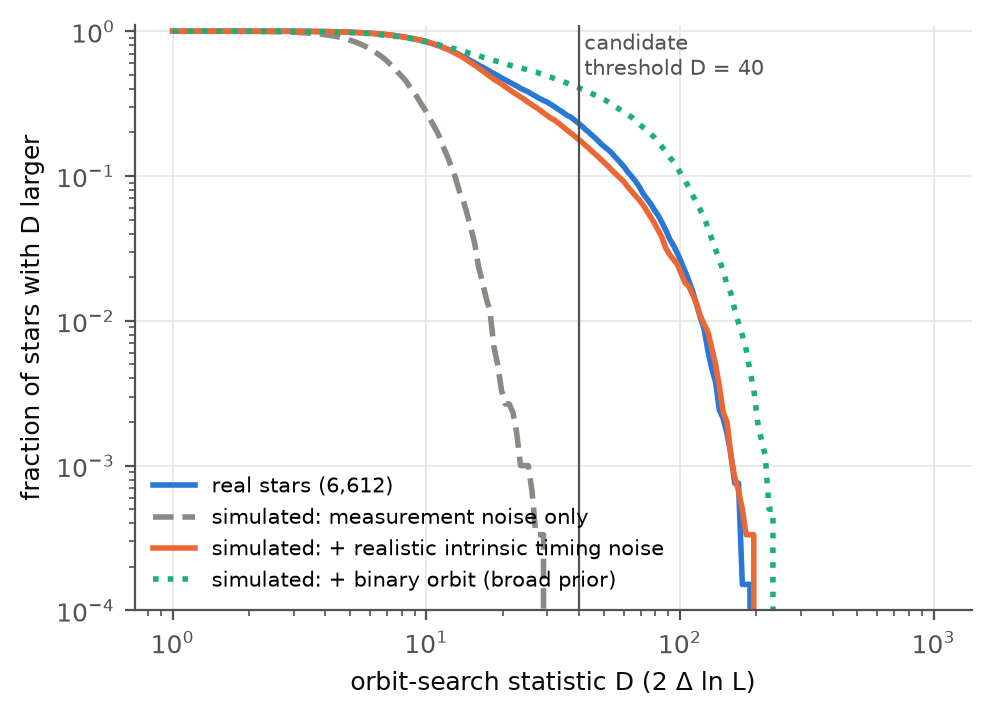
\includegraphics[width=0.66\textwidth]{fig_D_survival}
\caption{Fraction of stars with an orbit-search statistic above $D$: real stars (blue) and simulated stars of the same sample with
measurement noise only (grey), with realistic intrinsic timing noise (orange) and with injected orbits (green; broad
prior: $P=300$--$10^4$\,d, $M_2=0.05$--$1.5\,\Msun$, random inclination).}
\label{fig:D}
\end{figure}

\paragraph{Candidates vs noise.} At each cut the number of real stars is close to the number expected from intrinsic noise alone
(\cref{fig:funnel}). At $D>40$ the real stars exceed the noise model by 30\% (1{,}519 vs 1{,}172), an imperfection of the
noise model at moderate $D$, but after the cuts that select orbit-like signals the real count is \emph{below} the
expectation: \NCAND\ observed vs \EXPECTED\ expected. There is no excess of orbit-like signals.

\begin{figure}[ht]\centering
\fig{fig_funnel}{0.72}
\caption{Number of stars passing the successive cuts: real (blue) and expected from intrinsic timing noise alone (orange; the
simulated noise carries no amplitude variability, so the last step uses the real amplitude-stability pass rate of stars passing
the other cuts).}
\label{fig:funnel}
\end{figure}

\paragraph{Amplitudes.} The best-fit sinusoids of most stars are small (\cref{fig:amp}): typically 100--300\,s at periods of
1--3\,yr, set by the noise. The candidates lie at 300--3000\,s and 5--20\,yr, where the intrinsic wander is largest.

\begin{figure}[ht]\centering
\fig{fig_amp_period}{0.66}
\caption{Best-fit \OC\ semi-amplitude and period of every star (grey) and of the \NCAND\ candidates (blue), with the
light-travel amplitude of an edge-on companion of $0.1$, $0.4$ and $1.5\,\Msun$. The vertical stripes at long periods are
the period grid; values above the $1.5\,\Msun$ line and beyond $\sim$20\,yr are intrinsic wander or trends.}
\label{fig:amp}
\end{figure}

%==============================================================================
\section{Detection efficiency}\label{sec:efficiency}
The probability that a binary is flagged is measured by injection into the \emph{real} stars: for each of the 6{,}612 stars,
two Keplerian orbits are drawn ($P_{\rm orb}$ log-uniform 300--$10^4$\,d, $M_2$ log-uniform 0.05--1.5\,\Msun, $M_1=0.65\,\Msun$,
isotropic inclination, half circular and half with $e$ uniform in 0--0.7) and their light-travel delay is added to the star's
measured season delays in all bands; the search and the cuts are then rerun unchanged. The injected binaries therefore carry
each star's real intrinsic timing noise, real amplitude behaviour (so Blazhko-type stars are rejected exactly as in the data),
cadence and errors. The orbit is added at the season epochs, neglecting the smearing of the delay within a season (amplitude loss
$\lesssim$10\% at 1000\,d, $\lesssim$1\% at 3000\,d); \VALIDATION

\Cref{fig:eff} shows the result. For $0.4$--$1.5\,\Msun$ companions on 1{,}000--10{,}000-d orbits the efficiency is \EPS\ (\EPSRAW\ before the smearing correction; the earlier estimate from simulated stars without intrinsic timing noise, multiplied by the fraction of real stars with a steady amplitude, was \EPSOLD, close to the direct measurement); it falls
to \EPSLOWP\ at 300--1{,}000\,d (small amplitudes, season smearing) and is \EPSLOWM\ for $0.15$--$0.4\,\Msun$ at 3{,}000--10{,}000\,d.
Binaries are missed because their orbit is seen nearly face-on, because the host star varies in amplitude (Blazhko type; the
amplitude cut rejects it), or because the host's own timing noise distorts the signal.

\begin{figure}[ht]\centering
\fig{fig_efficiency}{0.66}
\caption{Probability that a binary is flagged as a candidate, from orbits injected into the real stars' timing data,
in bins of orbital period and companion mass (averaged over inclination and eccentricity; before the season-smearing correction, which lowers the values by 30\% below 1000\,d and $\le$6\% above). The values of 0.01--0.04 for low-mass companions are mostly stars that are flagged because of their own timing noise.}
\label{fig:eff}
\end{figure}

%==============================================================================
\section{Upper limit on the binary fraction}\label{sec:limit}
\paragraph{Argument.} Let a fraction $f$ of the $N=6{,}612$ stars have a companion from the injected population of a given
bin. The expected number of such binaries that are flagged is $f N \varepsilon$. We flag $k=\NCAND$ stars in total. Counting
\emph{every} one of them as a binary (no subtraction of noise candidates) we require $fN\varepsilon \le k_{95}$, where
$k_{95}=\KNINETYFIVE$ is the 95\% upper limit on a Poisson mean given $k$ observed, so
\begin{equation}
f < \frac{k_{95}}{N\,\varepsilon}.
\end{equation}
Binaries that are not flagged are allowed by construction: they are accounted for by $\varepsilon$. The argument does not depend
on the model of the intrinsic noise; it only needs the efficiency, which is measured on the real stars.

\paragraph{Result.} \Cref{tab:limits} and \cref{fig:limit}. If the \EXPECTED\ candidates expected from noise are subtracted, the
limit becomes much tighter (\FMAXBKG; \FMAXBKGHALF\ if the noise expectation is halved), but this depends on the noise model and
we do not adopt it.

\begin{table}[ht]\centering\small
\caption{95\% upper limits on the binary fraction of LMC RRab (6{,}612 stars with MACHO+OGLE data, 1992--2026).
$\varepsilon$: probability that a binary of the bin is flagged (from injections into the real stars; 68\% range from the
number of injections). $f_{\max}$: counting all candidates as binaries. $f_{\max}^{\rm bkg}$: noise candidates subtracted (model dependent).}
\label{tab:limits}
\TABLE
\end{table}

\begin{figure}[ht]\centering
\fig{fig_upper_limit}{0.66}
\caption{95\% upper limit on the binary fraction vs orbital period for three companion-mass ranges. Literature values are shown
for orientation; they refer to different methods and populations (\cref{sec:literature}).}
\label{fig:limit}
\end{figure}

\paragraph{Assumptions.} (i) The limit refers to the injected population within each bin (log-uniform period and mass, isotropic
orientation, $e<0.7$); a population concentrated where the efficiency is lower gives a weaker limit. (ii) Binarity is assumed
independent of the host's amplitude behaviour and intrinsic timing noise (the injections place orbits into randomly chosen real
stars). (iii) The sample is the MACHO-covered central LMC. (iv) Real stars could already contain undetected binaries; adding an
orbit to such a star can only increase its detectability, a negligible effect at $f\lesssim5\%$.

%==============================================================================
\section{Individual candidates and the blind test}\label{sec:candidates}
On 1 October 2026, before the OGLE data after 2016 were available, we froze orbit predictions for 2016--2026 for 28 candidates
from the data up to 2016, with the predictive uncertainty from the stars' red-noise model. The new data test them
(\cref{fig:blind}): 2 predictions were confirmed (13854, 15158), 20 failed and 5 were inconclusive (one star had no new data).
A failed prediction shows that the frozen best-fit orbit was wrong, not that the star is single; a passed one is evidence for a
coherent, orbit-like signal under the adopted noise model.

\begin{figure}[ht]\centering
\fig{fig_blind_test}{0.95}
\caption{Blind test. Points to the dotted line: data used for the prediction (MACHO $B$, $R$; OGLE $I$). Grey band: frozen orbit
prediction ($\pm2\sigma$). Orange: OGLE seasons 2017--2026. Left: 13854, confirmed. Right: 03269, failed.}
\label{fig:blind}
\end{figure}

A follow-up short list (12 stars) requires: a physically possible orbit (amplitude below an edge-on $2\,\Msun$ companion), at least
two orbital cycles in 34 years, a steady pulsation amplitude, and a successful prediction of the 2017--2026 data (blind for
13854 and 15158; not blind for stars first selected with the new data). \Cref{tab:short} lists them.

\begin{table}[ht]\centering\small
\caption{Follow-up short list. $P$, $e$: Keplerian fit to 1992--2026. $M_{2,\min}$: minimum companion mass ($M_1=0.65\,\Msun$,
edge-on). $K_1$: predicted radial-velocity semi-amplitude of the RR Lyrae.}
\label{tab:short}
\SHORTTABLE
\end{table}

%==============================================================================
\section{What timing can and cannot establish}\label{sec:limits_of_method}
\begin{itemize}[leftmargin=*]
\item A circular orbit produces a sinusoidal delay. A strictly periodic intrinsic phase modulation produces the same signal.
In simulations on the real cadences, circular orbits cannot be separated from such modulation (power $\le$13\% at 1\% false
alarm); strongly eccentric orbits ($e=0.5$, amplitude 8 season errors) can (93--97\%), because the Keplerian waveform is distinctive.
\item Such modulation exists: about 2.4\% of RR Lyrae show a periodic timing component beyond random wander, and some of these
are strictly coherent with amplitudes too large for any orbit. About 90\% of the coherent intrinsic modulators also vary in
pulsation amplitude, which an orbit does not do; this is why the amplitude-stability cut is central.
\item Consequently individual candidates remain candidates until radial velocities (semi-amplitudes 3--12\,\kms\ over years) or
Gaia epoch astrometry/photometry confirm them. The \emph{upper limit} is not affected: it counts all candidates as binaries.
\end{itemize}

%==============================================================================
\section{Comparison with the literature}\label{sec:literature}
\begin{itemize}[leftmargin=*]
\item \citet{Hajdu2015} found 20 probable light-travel-time binaries among 1{,}952 OGLE-III bulge RRab ($\sim$1\%), doubled
this for Blazhko stars and again for missed orbits, and concluded that $\gtrsim4\%$ of RR Lyrae are in binaries. This is a lower
estimate that assumes the candidates are real and covers all companion masses. Their raw candidate rate is close to ours
(\NCAND/6{,}612 = 1.4\%); our simulations show that such a rate is produced by intrinsic timing noise, so the candidates alone do
not establish a lower bound.
\item \citet{Hajdu2021} presented 87 bulge candidates with $P_{\rm orb}>1000$\,d and companion masses clustering near 0.6, 0.2 and
0.067\,\Msun; none has been confirmed or refuted since \citep{Salinas2026}.
\item \citet{Kervella2019} found proper-motion anomalies (Hipparcos vs Gaia DR2) in 13 of 198 nearby RR Lyrae, plus 61
candidates, and concluded that at least 7\% are binaries. That method is sensitive to different orbits and companion masses and
probes the solar neighbourhood.
\item \citet{Iorio2026} found no genuine RR Lyrae in the Gaia DR3 astrometric binary catalogues; for metal-rich disc RR Lyrae with
predicted orbits of $\sim$900--2000\,d, their fiducial models give an upper limit of $\approx$30\%. The LMC sample is mostly
metal-poor, so our limit does not test that binary-evolution channel \citep{Bobrick2024}.
\end{itemize}

%==============================================================================
\section{Reproducibility}\label{sec:repro}
Scripts (repository): \texttt{level1\_real.py}, \texttt{level2.py} (timing and search; run with \texttt{--ogle4 extended});
\texttt{level1\_sims.py} (light-curve simulations); \texttt{inject\_real.py} (efficiency); \texttt{upper\_limit\_v4.py} (limits,
\texttt{results/partB\_v4/upper\_limits.csv}); \texttt{shortlist\_v4.py}; \texttt{test\_frozen\_predictions.py} (blind test; frozen
inputs under git tag \texttt{predictions-2026-10-01}); \texttt{plot\_binary\_fraction.py} (figures). Tests: \texttt{pytest}.
Details and all intermediate numbers: \texttt{JOURNAL.md}.

%==============================================================================
\begin{thebibliography}{99}\small
\bibitem[Bobrick et al.(2024)]{Bobrick2024} Bobrick A., Iorio G., Belokurov V., et al., 2024, MNRAS, 527, 12196.
\url{https://doi.org/10.1093/mnras/stad3996}
\bibitem[Hajdu et al.(2015)]{Hajdu2015} Hajdu G., Catelan M., Jurcsik J., et al., 2015, MNRAS, 449, L113.
\url{https://doi.org/10.1093/mnrasl/slv024}, \url{https://arxiv.org/abs/1502.01318}
\bibitem[Hajdu et al.(2021)]{Hajdu2021} Hajdu G., et al., 2021, ApJ, 915, 50. \url{https://doi.org/10.3847/1538-4357/abff4b},
\url{https://arxiv.org/abs/2105.03750}
\bibitem[Iorio et al.(2026)]{Iorio2026} Iorio G., Nagarajan P., Bobrick A., et al., 2026, A\&A, 712, A223.
\url{https://doi.org/10.1051/0004-6361/202659978}, \url{https://arxiv.org/abs/2603.20429}
\bibitem[Kervella et al.(2019)]{Kervella2019} Kervella P., Gallenne A., Evans N.\,R., et al., 2019, A\&A, 623, A116.
\url{https://doi.org/10.1051/0004-6361/201834210}, \url{https://arxiv.org/abs/1811.08902}
\bibitem[Mr\'oz et al.(2024)]{Mroz2024} Mr\'oz P., Udalski A., Szyma\'nski M.\,K., et al., 2024, ApJL, 976, L19.
\url{https://doi.org/10.3847/2041-8213/ad8e68}
\bibitem[Salinas et al.(2026)]{Salinas2026} Salinas R., Kalari V., Hajdu G., Prudil Z., et al., 2026, arXiv:2603.28684.
\url{https://arxiv.org/abs/2603.28684}
\bibitem[Soszy\'nski et al.(2009)]{Soszynski2009} Soszy\'nski I., et al., 2009, AcA, 59, 1. \url{https://arxiv.org/abs/0903.2482}
\bibitem[Soszy\'nski et al.(2016)]{Soszynski2016} Soszy\'nski I., et al., 2016, AcA, 66, 131. \url{https://arxiv.org/abs/1606.02727}
\end{thebibliography}

\end{document}
